\documentclass[a4paper,12pt]{article}
% -------------------------------------------------
% Configuração de página
% -------------------------------------------------
\usepackage[a4paper,top=3cm,bottom=2cm,left=3cm,right=2cm]{geometry}
% -------------------------------------------------
% Codificação e idioma
% -------------------------------------------------
\usepackage[T1]{fontenc}
\usepackage[utf8]{inputenc}
\usepackage[english,brazil]{babel}
% -------------------------------------------------
% Pacotes matemáticos e fontes
% -------------------------------------------------
\usepackage{amsmath}
\usepackage{amsfonts}
\usepackage{amstext}
\usepackage{mathptmx}
% -------------------------------------------------
% Formatação geral
% -------------------------------------------------
\usepackage{indentfirst}
\usepackage{microtype}
\usepackage{setspace}
\onehalfspacing
\setlength{\parindent}{1.25cm}
\setlength{\parskip}{0pt}
% -------------------------------------------------
% Gráficos, tabelas e quadros
% -------------------------------------------------
\usepackage[table,xcdraw]{xcolor}
\usepackage{graphicx}
\usepackage{pgfplots}
\pgfplotsset{compat=1.18}
\usepackage{float}
\usepackage{booktabs}
\usepackage{array}
\usepackage{tabularx}
\usepackage{longtable}
\usepackage{multirow}
\usepackage{makecell}
\usepackage{threeparttable}
\usepackage[format=hang]{caption}
\captionsetup[quadro]{justification=centering}
% -------------------------------------------------
% Quadros (ambiente próprio)
% -------------------------------------------------
\usepackage{tocloft}
\floatstyle{plaintop}
\newfloat{quadro}{htbp}{loq}
\floatname{quadro}{Quadro}
\newcommand{\listofquadros}{
    \listof{quadro}{Lista de Quadros}
}
% -------------------------------------------------
% Outros pacotes
% -------------------------------------------------
\usepackage{enumerate}
\usepackage{nomencl}
\usepackage{verbatim}
\usepackage{hyperref}
\usepackage[alf]{abntex2cite}
\usepackage{tcolorbox}
\usepackage{fancyhdr}
\usepackage{appendix}
\usepackage{multicol}
\usepackage{adjustbox}
\usepackage{wasysym}
\usepackage{pdflscape}
\newcommand{\fonte}[1]{\par\noindent\footnotesize Fonte: #1}
\newcommand{\nota}[1]{\par\noindent\footnotesize Nota: #1}
\newcommand{\celula}[1]{\makecell[l]{#1}}
% -------------------------------------------------
% Listagem de código-fonte
% -------------------------------------------------
\usepackage{listings}
\renewcommand{\lstlistingname}{Código}
\renewcommand{\lstlistlistingname}{Lista de Códigos}
% -------------------------------------------------
% Acentuação em listagens
% -------------------------------------------------
\lstset{
    basicstyle=\ttfamily\small,
    numbers=left,
    numberstyle=\tiny,
    stepnumber=1,
    numbersep=8pt,
    frame=single,
    breaklines=true,
    tabsize=4,
    showstringspaces=false,
    captionpos=b,
    keywordstyle=\color{blue},
    commentstyle=\color{green!50!black},
    stringstyle=\color{red!70!black},
    literate=
      {á}{{\\'a}}1 {à}{{\\\`a}}1 {ã}{{\\\~a}}1 {â}{{\\^a}}1
      {é}{{\\'e}}1 {ê}{{\\^e}}1
      {í}{{\\'i}}1
      {ó}{{\\'o}}1 {õ}{{\\\~o}}1 {ô}{{\\^o}}1
      {ú}{{\\'u}}1
      {ç}{{\c{c}}}1
      {Á}{{\\'A}}1 {À}{{\\\`A}}1 {Ã}{{\\\~A}}1 {Â}{{\\^A}}1
      {É}{{\\'E}}1 {Ê}{{\\^E}}1
      {Í}{{\\'I}}1
      {Ó}{{\\'O}}1 {Õ}{{\\\~O}}1 {Ô}{{\\^O}}1
      {Ú}{{\\'U}}1
      {Ç}{{\c{C}}}1
}

\hypersetup{
    hidelinks,
    pdfborder={0 0 0}
}

% -------------------------------------------------
% Documento
% -------------------------------------------------
\begin{document}
% -------------------------------------------------
% Folha de rosto
% -------------------------------------------------
\begin{titlepage}
    \thispagestyle{empty}
    \begin{center}
        % Logos
        \begin{minipage}{0.22\textwidth}
            \centering
            \includegraphics[width=0.9\linewidth]{figuras/ufs\_logo.png}
        \end{minipage}
        \hspace{1.5cm}
        \begin{minipage}{0.22\textwidth}
            \centering
            \includegraphics[width=0.9\linewidth]{figuras/ppgdem\_logo.png}
        \end{minipage}
        \par
        \vspace{1.2cm}
        % Instituições
        {\large UNIVERSIDADE FEDERAL DE SERGIPE\par}
        {\large UNIVERSIDADE FEDERAL DO RIO GRANDE DO NORTE\par}
        \vspace{0.5cm}
        {\large PROGRAMA DE PÓS-GRADUAÇÃO EM DEMOGRAFIA\par}
        {\large DOUTORADO INTERINSTITUCIONAL EM POPULAÇÃO,\par}
        {\large ESTATÍSTICAS SOCIAIS E POLÍTICAS PÚBLICAS\par}
        \vspace{3cm}
        % Nome do aluno
        {\large \textbf{Andrés Ignácio Martínez Menéndez}\par}
        \vspace{3cm}
        % Título
        {\Large \textbf{Componentes da Dinâmica Demográfica}\par}
        \vspace{0.6cm}
        {\large Laboratório de Análise de Dados Demográficos\par}
        \vfill
        % Local e data
        {\small Aracaju (SE)\par}
        {\small Novembro de 2026\par}
    \end{center}
\end{titlepage}
\clearpage

% -------------------------------------------------
% Sumário
% -------------------------------------------------
\renewcommand{\contentsname}{\centering SUMÁRIO}
\tableofcontents
\thispagestyle{empty}
\clearpage

\renewcommand{\listfigurename}{\centering LISTA DE FIGURAS}
\listoffigures
\thispagestyle{empty}
\clearpage

\renewcommand{\listtablename}{\centering LISTA DE TABELAS}
\listoftables
\thispagestyle{empty}
\clearpage

\pagenumbering{arabic}


\section{Introdução}

O Censo Demográfico constitui uma fonte central para descrever as condições de vida e a composição da população brasileira em diferentes escalas territoriais. Seus dados permitem examinar, além do tamanho e da estrutura por sexo e idade, dimensões relacionadas ao trabalho, à educação, aos rendimentos e às condições dos domicílios. A divulgação de informações para os municípios torna possível observar desigualdades que podem ficar encobertas por indicadores agregados para o estado ou para o país \cite{ibge2022censo}.

Este trabalho analisa indicadores sociodemográficos dos municípios de Sergipe com base nos microdados do Censo Demográfico 2022. Na dimensão populacional, são estimadas a razão de sexo, a taxa de desocupação, a taxa de analfabetismo entre pessoas de 15 a 64 anos e as médias e participações relativas dos rendimentos do trabalho e de outras fontes. Também se examina como esses indicadores variam entre os municípios e como se associam à participação de ocupações do setor primário. A razão de sexo é tratada como uma medida da composição da população; sua distribuição municipal, por si só, não permite atribuir diferenças observadas exclusivamente à migração.

Na dimensão domiciliar, o estudo descreve a proporção de domicílios cuja pessoa responsável é mulher, a renda domiciliar per capita segundo o sexo dessa pessoa e as diferenças de renda entre os grupos. São examinadas ainda as condições de acesso à água canalizada, ao esgotamento sanitário e à internet. As estimativas são organizadas por município, permitindo identificar contrastes territoriais e discutir em que medida os padrões observados se relacionam com as condições de trabalho e renda.

O objetivo é construir um retrato comparativo das condições demográficas, econômicas e domiciliares dos municípios sergipanos, articulando indicadores e associações estatísticas sugeridas pelo trabalho da disciplina. Os resultados descrevem relações observadas nos dados censitários de 2022 e não devem ser interpretados, isoladamente, como evidência de causalidade. Após a apresentação dos dados e procedimentos, o texto discute os indicadores demográficos e, em seguida, os indicadores domiciliares, encerrando com uma síntese dos principais achados. O script em R que gera os resultados está disponível, bem como os arquivos .rds e os próprios arquivos Latex, estão no repositório online: \url{https://github.com/ammenendez/cdd-lab01.git}.


\section{Resultados}

\subsection{Indicadores demográficos}

\subsubsection{Razão de sexo: municípios com maior predominância masculina e feminina}

A razão de sexo foi calculada como o número de homens para cada 100 mulheres. Valores superiores a 100 indicam predominância masculina, enquanto valores inferiores a 100 indicam predominância feminina. A Tabela~\ref{tab:razao-sexo-top10} apresenta os dez municípios com maior predominância de cada sexo.

\begin{table}[htbp]
\centering
\caption{Dez municípios com maior predominância masculina e feminina, Sergipe, 2022}
\label{tab:razao-sexo-top10}
\small
\begin{tabular}{r l l r}
\toprule
Posição & Município & Predominância & Homens por 100 mulheres \\
\midrule
\multicolumn{4}{l}{\textbf{Maior predominância masculina}} \\
1 & Canhoba & Masculina & 106,71 \\
2 & Gararu & Masculina & 106,17 \\
3 & Itabi & Masculina & 102,95 \\
4 & Brejo Grande & Masculina & 102,77 \\
5 & Poço Redondo & Masculina & 102,32 \\
6 & Porto da Folha & Masculina & 101,90 \\
7 & Areia Branca & Masculina & 101,82 \\
8 & Japoatã & Masculina & 101,70 \\
9 & Santa Rosa de Lima & Masculina & 101,59 \\
10 & Gracho Cardoso & Masculina & 101,38 \\
\midrule
\multicolumn{4}{l}{\textbf{Maior predominância feminina}} \\
1 & Aracaju & Feminina & 84,81 \\
2 & Rosário do Catete & Feminina & 87,89 \\
3 & General Maynard & Feminina & 89,22 \\
4 & Nossa Senhora do Socorro & Feminina & 90,11 \\
5 & Carmópolis & Feminina & 91,13 \\
6 & Estância & Feminina & 91,48 \\
7 & Umbaúba & Feminina & 91,80 \\
8 & Barra dos Coqueiros & Feminina & 91,83 \\
9 & Laranjeiras & Feminina & 91,95 \\
10 & Propriá & Feminina & 91,97 \\
\bottomrule
\end{tabular}
\fonte{Elaboração própria com base nos microdados do Censo Demográfico 2022.}
\nota{Razão de sexo calculada como o número de homens para cada 100 mulheres.}
\end{table}


\subsubsection{Razão de sexo e participação do setor primário}

Para avaliar se os municípios com menor razão de sexo são também aqueles mais baseados em atividades do setor primário, comparamos a razão de sexo municipal com a proporção de pessoas ocupadas cuja atividade principal pertence à agricultura, pecuária, produção florestal, pesca e aquicultura. A Figura~\ref{fig:razao-sexo-setor-primario} mostra a distribuição dos municípios e a tendência linear; o resultado da correlação de Pearson é apresentado a seguir.

A correlação de Pearson entre a razão de sexo e a proporção de ocupados no setor primário, calculada para 75 municípios, foi $r = 0{,}678$. O coeficiente positivo indica que municípios com razão de sexo mais alta tendem a apresentar maior proporção de ocupados no setor primário. Assim, os resultados não sustentam que os municípios com menor razão de sexo sejam justamente aqueles mais baseados no setor primário. A associação é municipal e descritiva e não demonstra causalidade.


\begin{figure}[htbp]
    \centering
    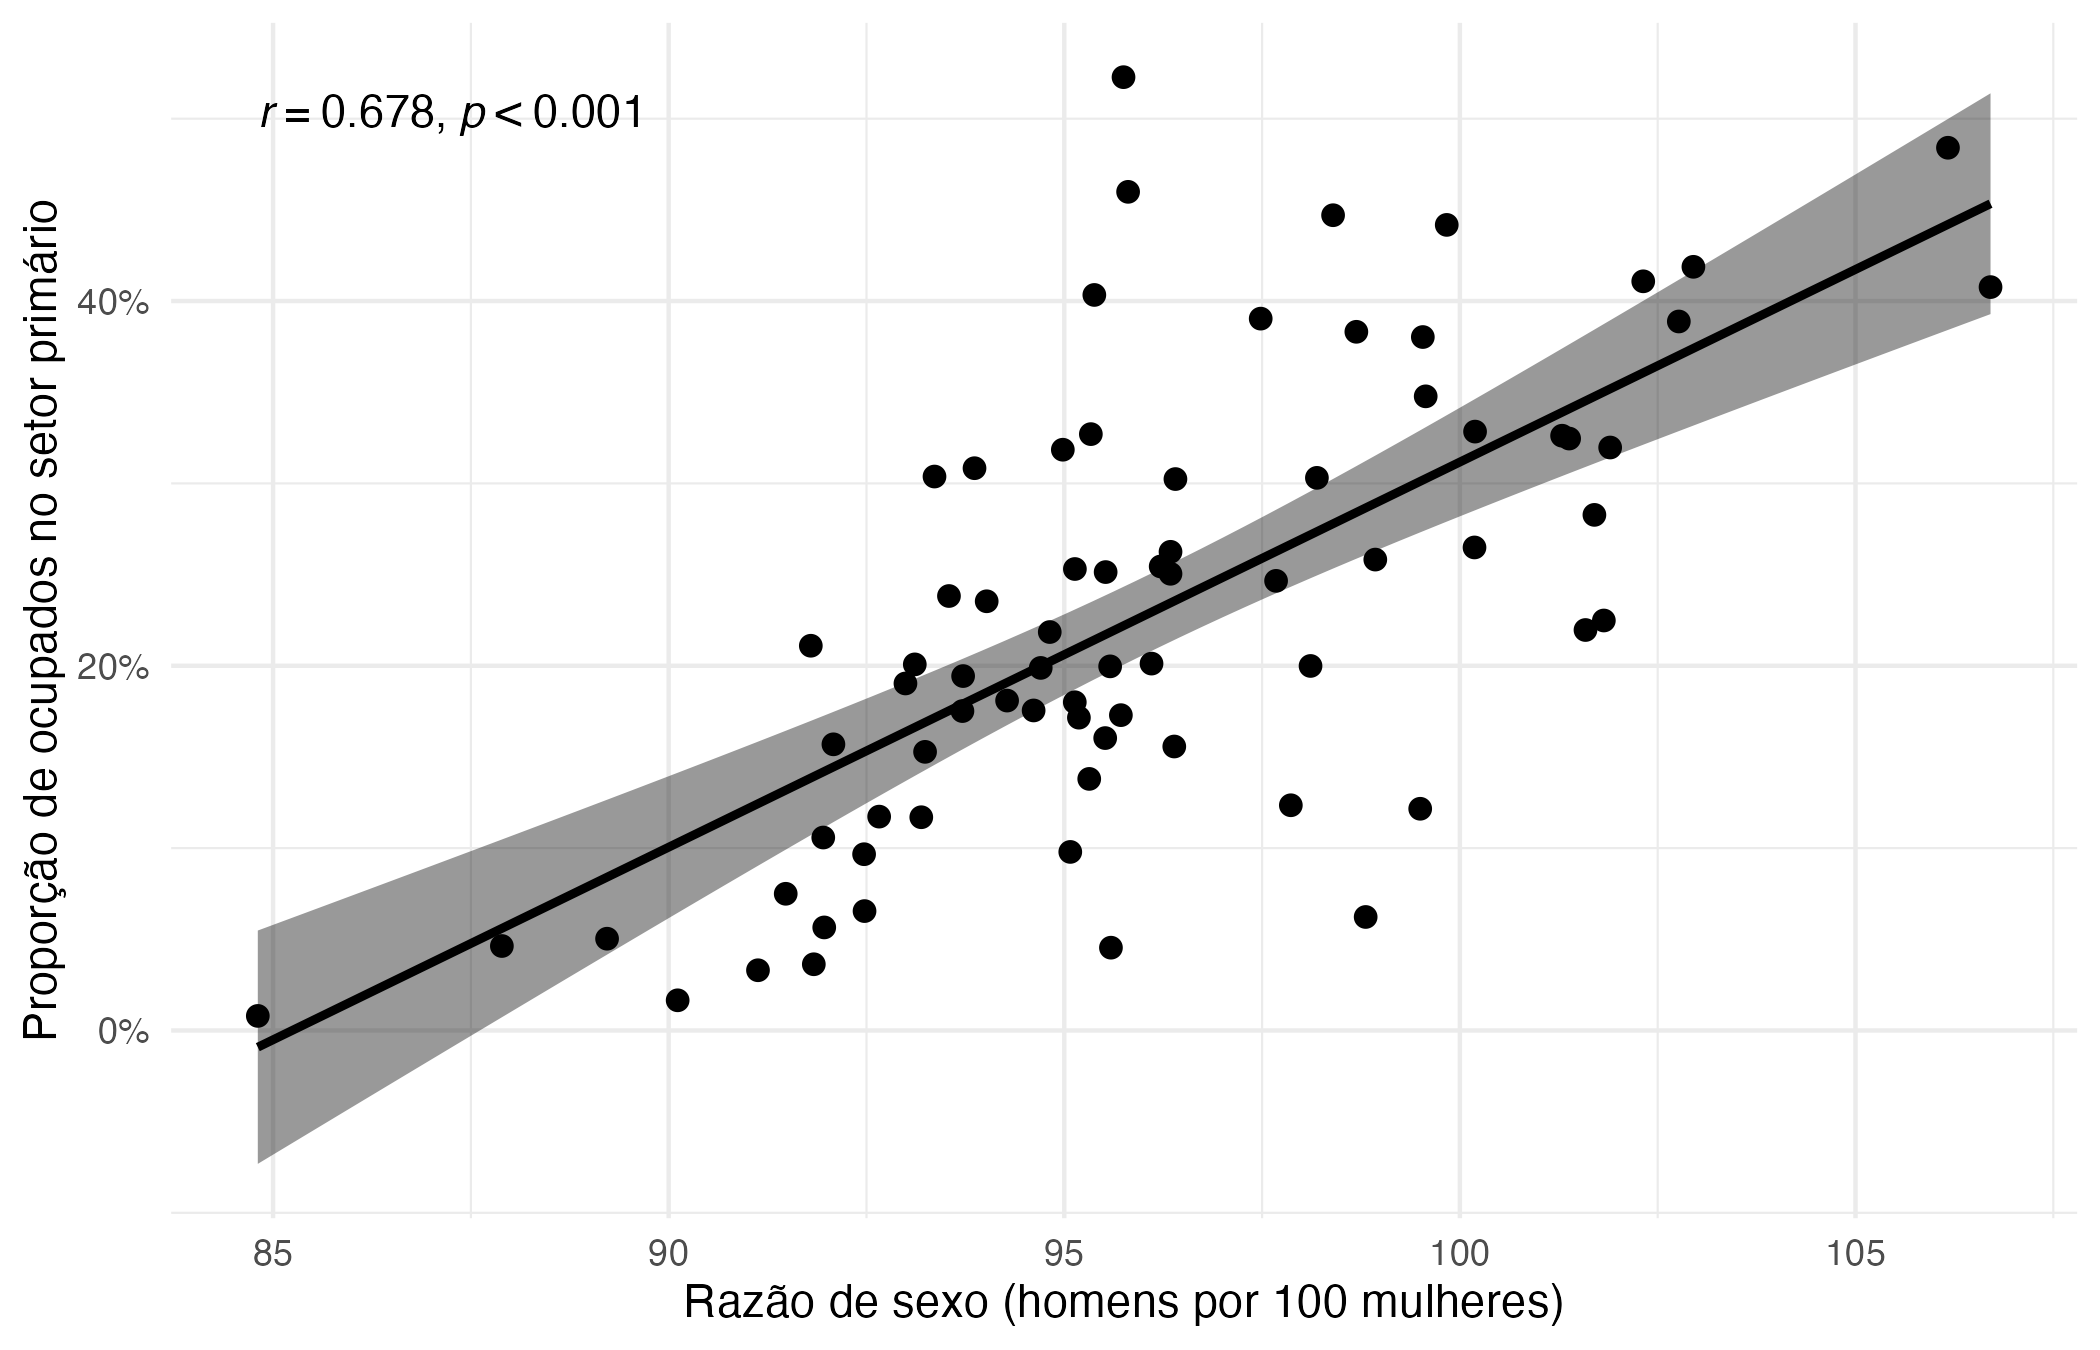
\includegraphics[width=0.9\textwidth]{resultados/item_1b_dispersao.png}
    \caption{Razão de sexo e proporção de ocupados no setor primário por município, Sergipe, 2022}
    \label{fig:razao-sexo-setor-primario}
    \fonte{Elaboração própria com base nos microdados do Censo Demográfico 2022.}
    \nota{A linha representa o ajuste linear e a faixa sombreada, seu intervalo de confiança de 95\%.}
\end{figure}

\subsection{Desocupação e nível de ocupação}

Para estimar a taxa de desocupação, consideramos as pessoas de 14 anos ou mais na força de trabalho (P0930 = 1). Nesse grupo, a categoria registrada como “não ocupada” em P0950 corresponde à pessoa desocupada: não tinha trabalho na semana de referência, tomou providências para consegui-lo no mês de referência e estava disponível para assumi-lo na semana de referência. Assim, a taxa de desocupação tem como denominador a força de trabalho, formada por ocupados e desocupados.

Essa medida não deve ser confundida com a proporção de pessoas não ocupadas. A categoria “não ocupada” também abrange pessoas fora da força de trabalho, que não estavam trabalhando nem procurando trabalho. Para representar o nível de ocupação, calculamos a proporção de pessoas ocupadas entre a população de 14 anos ou mais (P0920 = 1), usando P0960. Portanto, a taxa de ocupação e a taxa de desocupação têm denominadores diferentes e não são complementares \cite{ibgedicmicrodados2022}.

\begin{table}[H]
\centering
\caption{Três municípios com maiores e menores taxas de desocupação, Sergipe, 2022}
\label{tab:item2-taxa-desocupacao}
\small
\begin{tabular}{l r}
\toprule
\multicolumn{2}{l}{\textbf{Maiores taxas}} \\
Município & Taxa de desocupação (\%) \\
\midrule
Aquidabã & 19,59 \\
Cumbe & 19,44 \\
Carmópolis & 18,01 \\
\midrule
\multicolumn{2}{l}{\textbf{Menores taxas}} \\
Município & Taxa de desocupação (\%) \\
\midrule
Itabi & 2,38 \\
Gracho Cardoso & 2,40 \\
Macambira & 3,16 \\
\bottomrule
\end{tabular}
\begingroup
\fonte{Elaboração própria com base nos microdados do Censo Demográfico 2022.}
\nota{Taxa calculada como pessoas desocupadas entre as pessoas de 14 anos ou mais na força de trabalho (P0930=1).}\par
\endgroup
\end{table}

A Tabela~\ref{tab:item2-taxa-desocupacao} destaca os três municípios com maiores e menores taxas. No conjunto dos municípios, a taxa de desocupação variou de 2,38\% em Itabi a 19,59\% em Aquidabã.


\subsubsection{Nível de ocupação e participação do setor primário}

Comparamos a taxa de ocupação da população de 14 anos ou mais com a proporção de ocupados no setor primário, estimada a partir da atividade principal informada em P1030. A Figura~\ref{fig:item2-ocupacao-setor-primario} mostra a distribuição municipal e a tendência linear; o coeficiente de Pearson resume a associação entre os indicadores.

A correlação de Pearson entre a taxa de ocupação da população de 14 anos ou mais e a proporção de ocupados no setor primário, calculada para 75 municípios, foi $r = -0{,}287$. A associação observada é negativa e de magnitude modesta: municípios com maior taxa de ocupação tendem a apresentar menor participação relativa do setor primário entre os ocupados. Essa relação municipal é descritiva e não demonstra causalidade.


\begin{figure}[htbp]
    \centering
    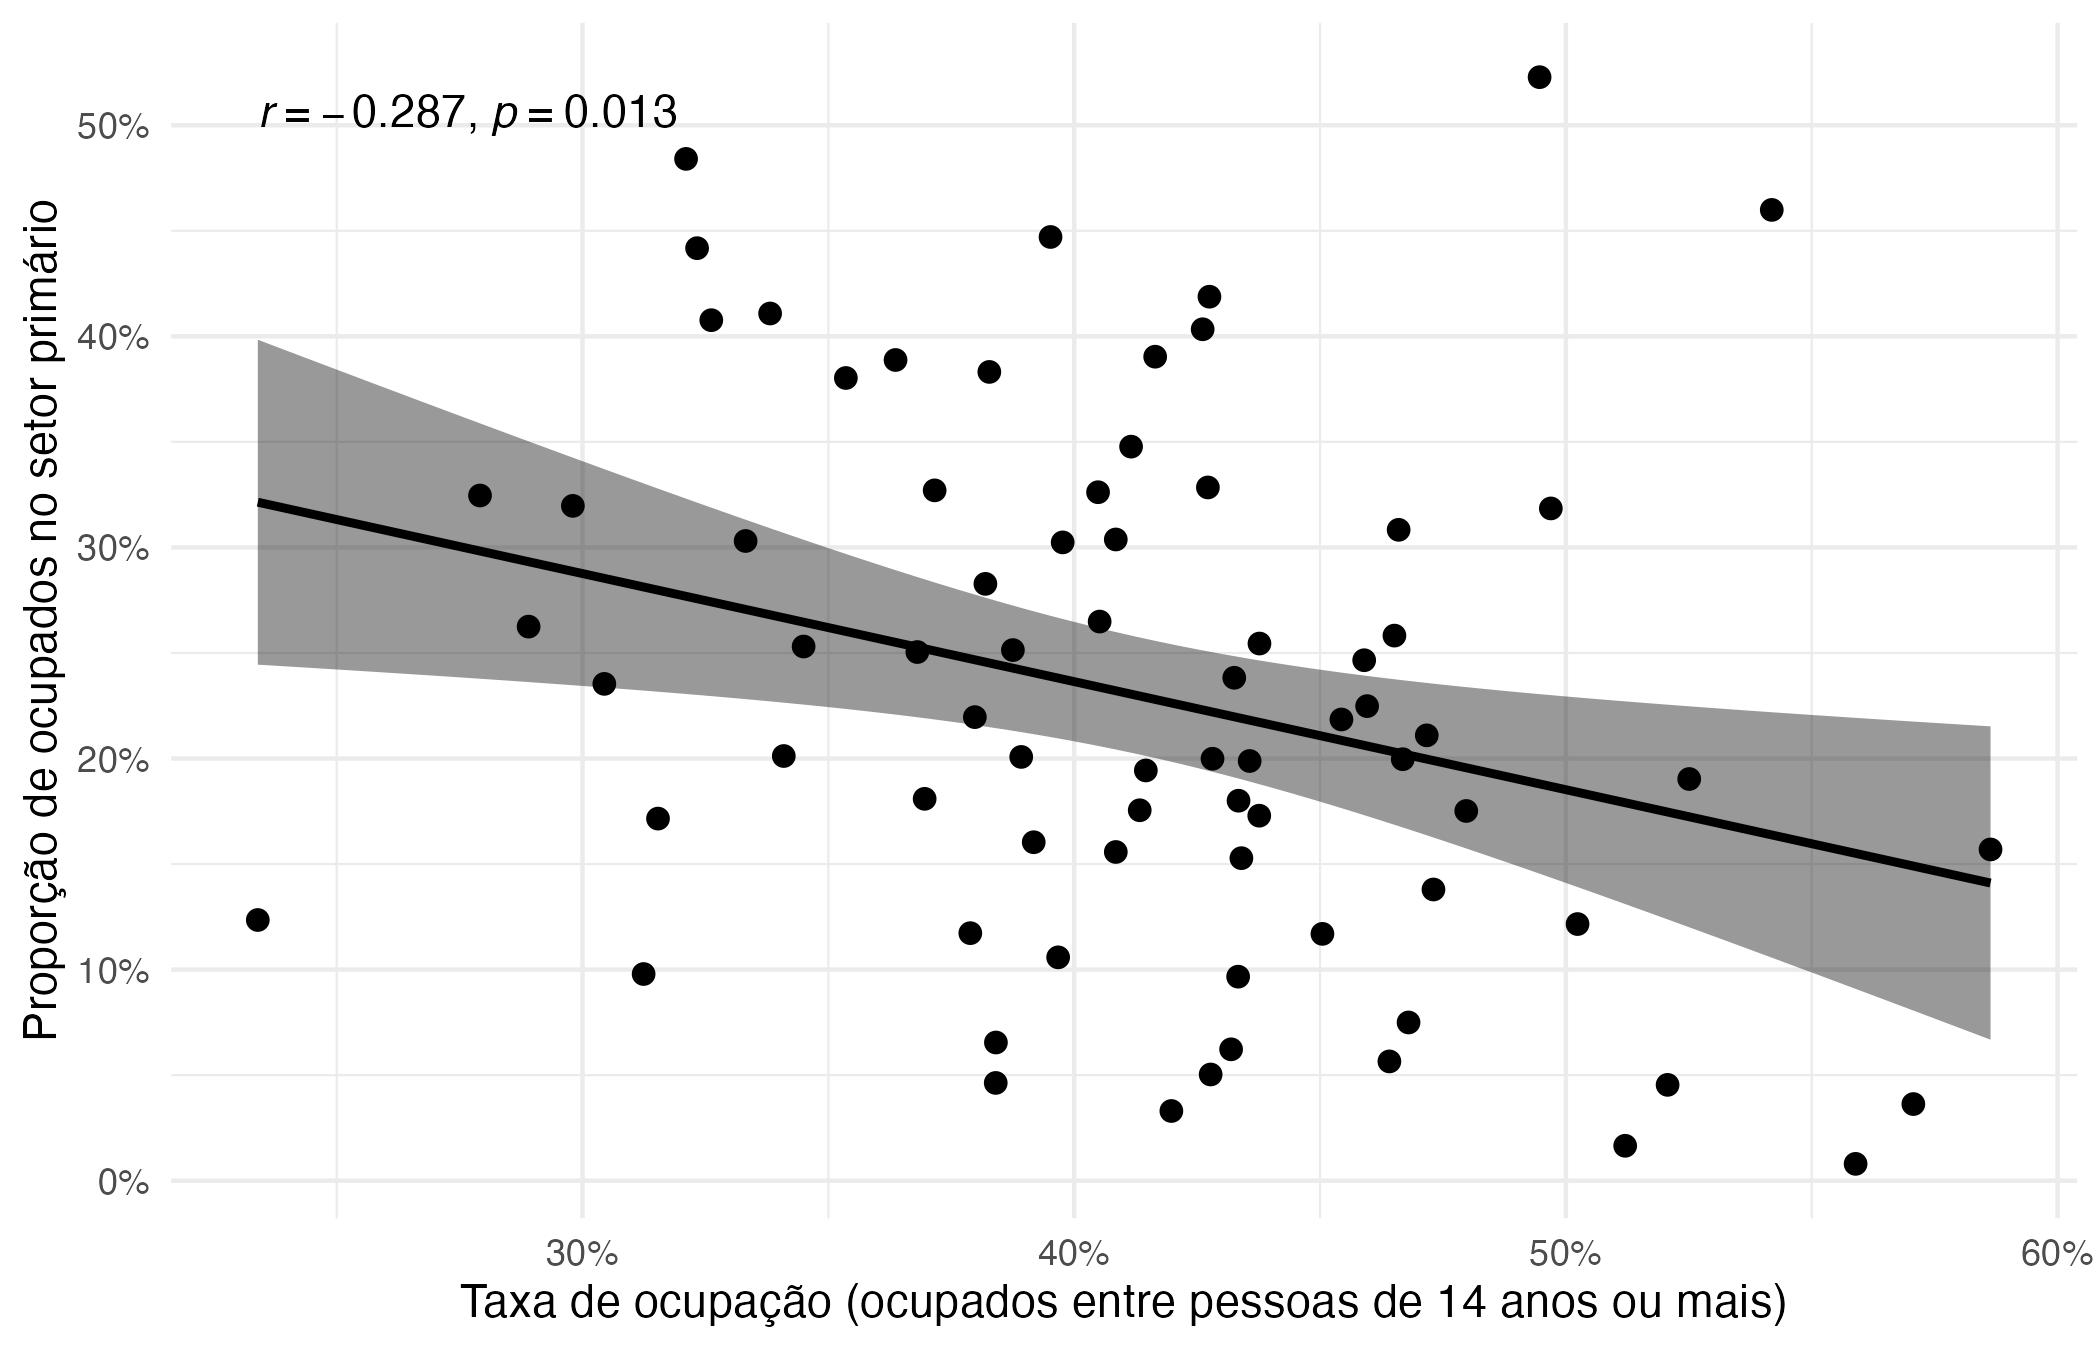
\includegraphics[width=0.9\textwidth]{resultados/item_2b_ocupacao_setor_primario.png}
    \caption{Taxa de ocupação e proporção de ocupados no setor primário por município, Sergipe, 2022}
    \label{fig:item2-ocupacao-setor-primario}
    \fonte{Elaboração própria com base nos microdados do Censo Demográfico 2022.}
    \nota{A linha representa o ajuste linear e a faixa sombreada, seu intervalo de confiança de 95\%.}
\end{figure}



\subsection{Taxa de analfabetismo}

Estimamos a taxa de analfabetismo entre as pessoas de 15 a 64 anos, considerando analfabeta a pessoa cuja resposta a P0640 foi “Não”. No Censo, alfabetização corresponde à capacidade de ler e escrever um bilhete simples no idioma conhecido. A Tabela~\ref{tab:item3-analfabetismo} apresenta os três municípios com taxas mais altas e mais baixas, além da estimativa ponderada para o conjunto de Sergipe \cite{ibgedicmicrodados2022}.

A taxa estadual de analfabetismo entre as pessoas de 15 a 64 anos foi 9,01\%. A taxa municipal mais alta foi registrada em Tomar do Geru (19,72\%); a mais baixa, em Aracaju (3,32\%).

\begin{table}[H]
\centering
\caption{Municípios com maiores e menores taxas de analfabetismo e estimativa estadual, população de 15 a 64 anos, Sergipe, 2022}
\label{tab:item3-analfabetismo}
\small
\begin{tabular}{l r}
\toprule
\multicolumn{2}{l}{\textbf{Maiores taxas municipais}} \\
Município & Taxa de analfabetismo (\%) \\
\midrule
Tomar do Geru & 19,72 \\
Gararu & 18,60 \\
Brejo Grande & 18,59 \\
\midrule
\multicolumn{2}{l}{\textbf{Menores taxas municipais}} \\
Município & Taxa de analfabetismo (\%) \\
\midrule
Aracaju & 3,32 \\
Barra dos Coqueiros & 3,62 \\
Nossa Senhora do Socorro & 5,06 \\
\midrule
\textbf{Estimativa estadual (Sergipe)} & 
9,01
 \\
\bottomrule
\end{tabular}
\begingroup
\fonte{Elaboração própria com base nos microdados do Censo Demográfico 2022.}
\nota{Pessoas de 15 a 64 anos; estimativas municipais e estadual ponderadas. A estimativa estadual foi calculada diretamente para Sergipe, não pela média simples das taxas municipais.}\par
\endgroup
\end{table}


\subsection{Rendimento por fonte}

Para os itens 4a e 4b do laboratório, usamos as médias municipais de rendimento do trabalho (P1080), de transferências e outras fontes (P1100) e do rendimento total (P1110). A Tabela~\ref{tab:item4-renda-fontes} resume os três municípios com maiores e menores médias de rendimento total e apresenta a participação percentual do trabalho e das transferências nesse total. A relação entre o rendimento de outras fontes e o rendimento total é ilustrada na Figura~\ref{fig:item4-renda-transferencias}.

A correlação de Pearson entre o rendimento médio de transferências e o rendimento médio total entre os municípios foi 0,16. Essa associação é positiva, mas fraca: municípios com maior rendimento médio de transferências tendem a apresentar rendimento médio total um pouco maior, embora haja bastante variação entre eles. A correlação descreve uma associação municipal e, por si só, não demonstra que as transferências causam o aumento do rendimento total nem que municípios com maior renda dependam mais delas.

\begin{table}[htbp]
\centering
\caption{Médias de rendimento por fonte nos municípios com maiores e menores rendimentos totais, Sergipe, 2022}
\label{tab:item4-renda-fontes}
\scriptsize
\begin{tabular}{lrrrrr}
\toprule
Município & Trabalho (R\$) & Transferências (R\$) & Total (R\$) & Trabalho (\%) & Transferências (\%) \\
\midrule
\multicolumn{6}{l}{\textbf{Maiores médias de rendimento total}} \\
Aracaju & 3.371,02 & 205,71 & 3.576,73 & 94,25 & 5,75 \\
Barra dos Coqueiros & 2.784,52 & 152,94 & 2.937,46 & 94,79 & 5,21 \\
São Cristóvão & 1.998,48 & 117,16 & 2.115,64 & 94,46 & 5,54 \\
\midrule
\multicolumn{6}{l}{\textbf{Menores médias de rendimento total}} \\
Ilha das Flores & 975,29 & 99,38 & 1.074,66 & 90,75 & 9,25 \\
Santa Luzia do Itanhy & 957,07 & 113,26 & 1.070,34 & 89,42 & 10,58 \\
Tomar do Geru & 858,82 & 130,92 & 989,74 & 86,77 & 13,23 \\
\bottomrule
\end{tabular}
\fonte{Elaboração própria com base nos microdados do Censo Demográfico 2022.}
\nota{As médias e participações são as estimadas pelo código para os registros válidos conjuntamente nas três variáveis de rendimento.}
\end{table}


\begin{figure}[H]
    \centering
    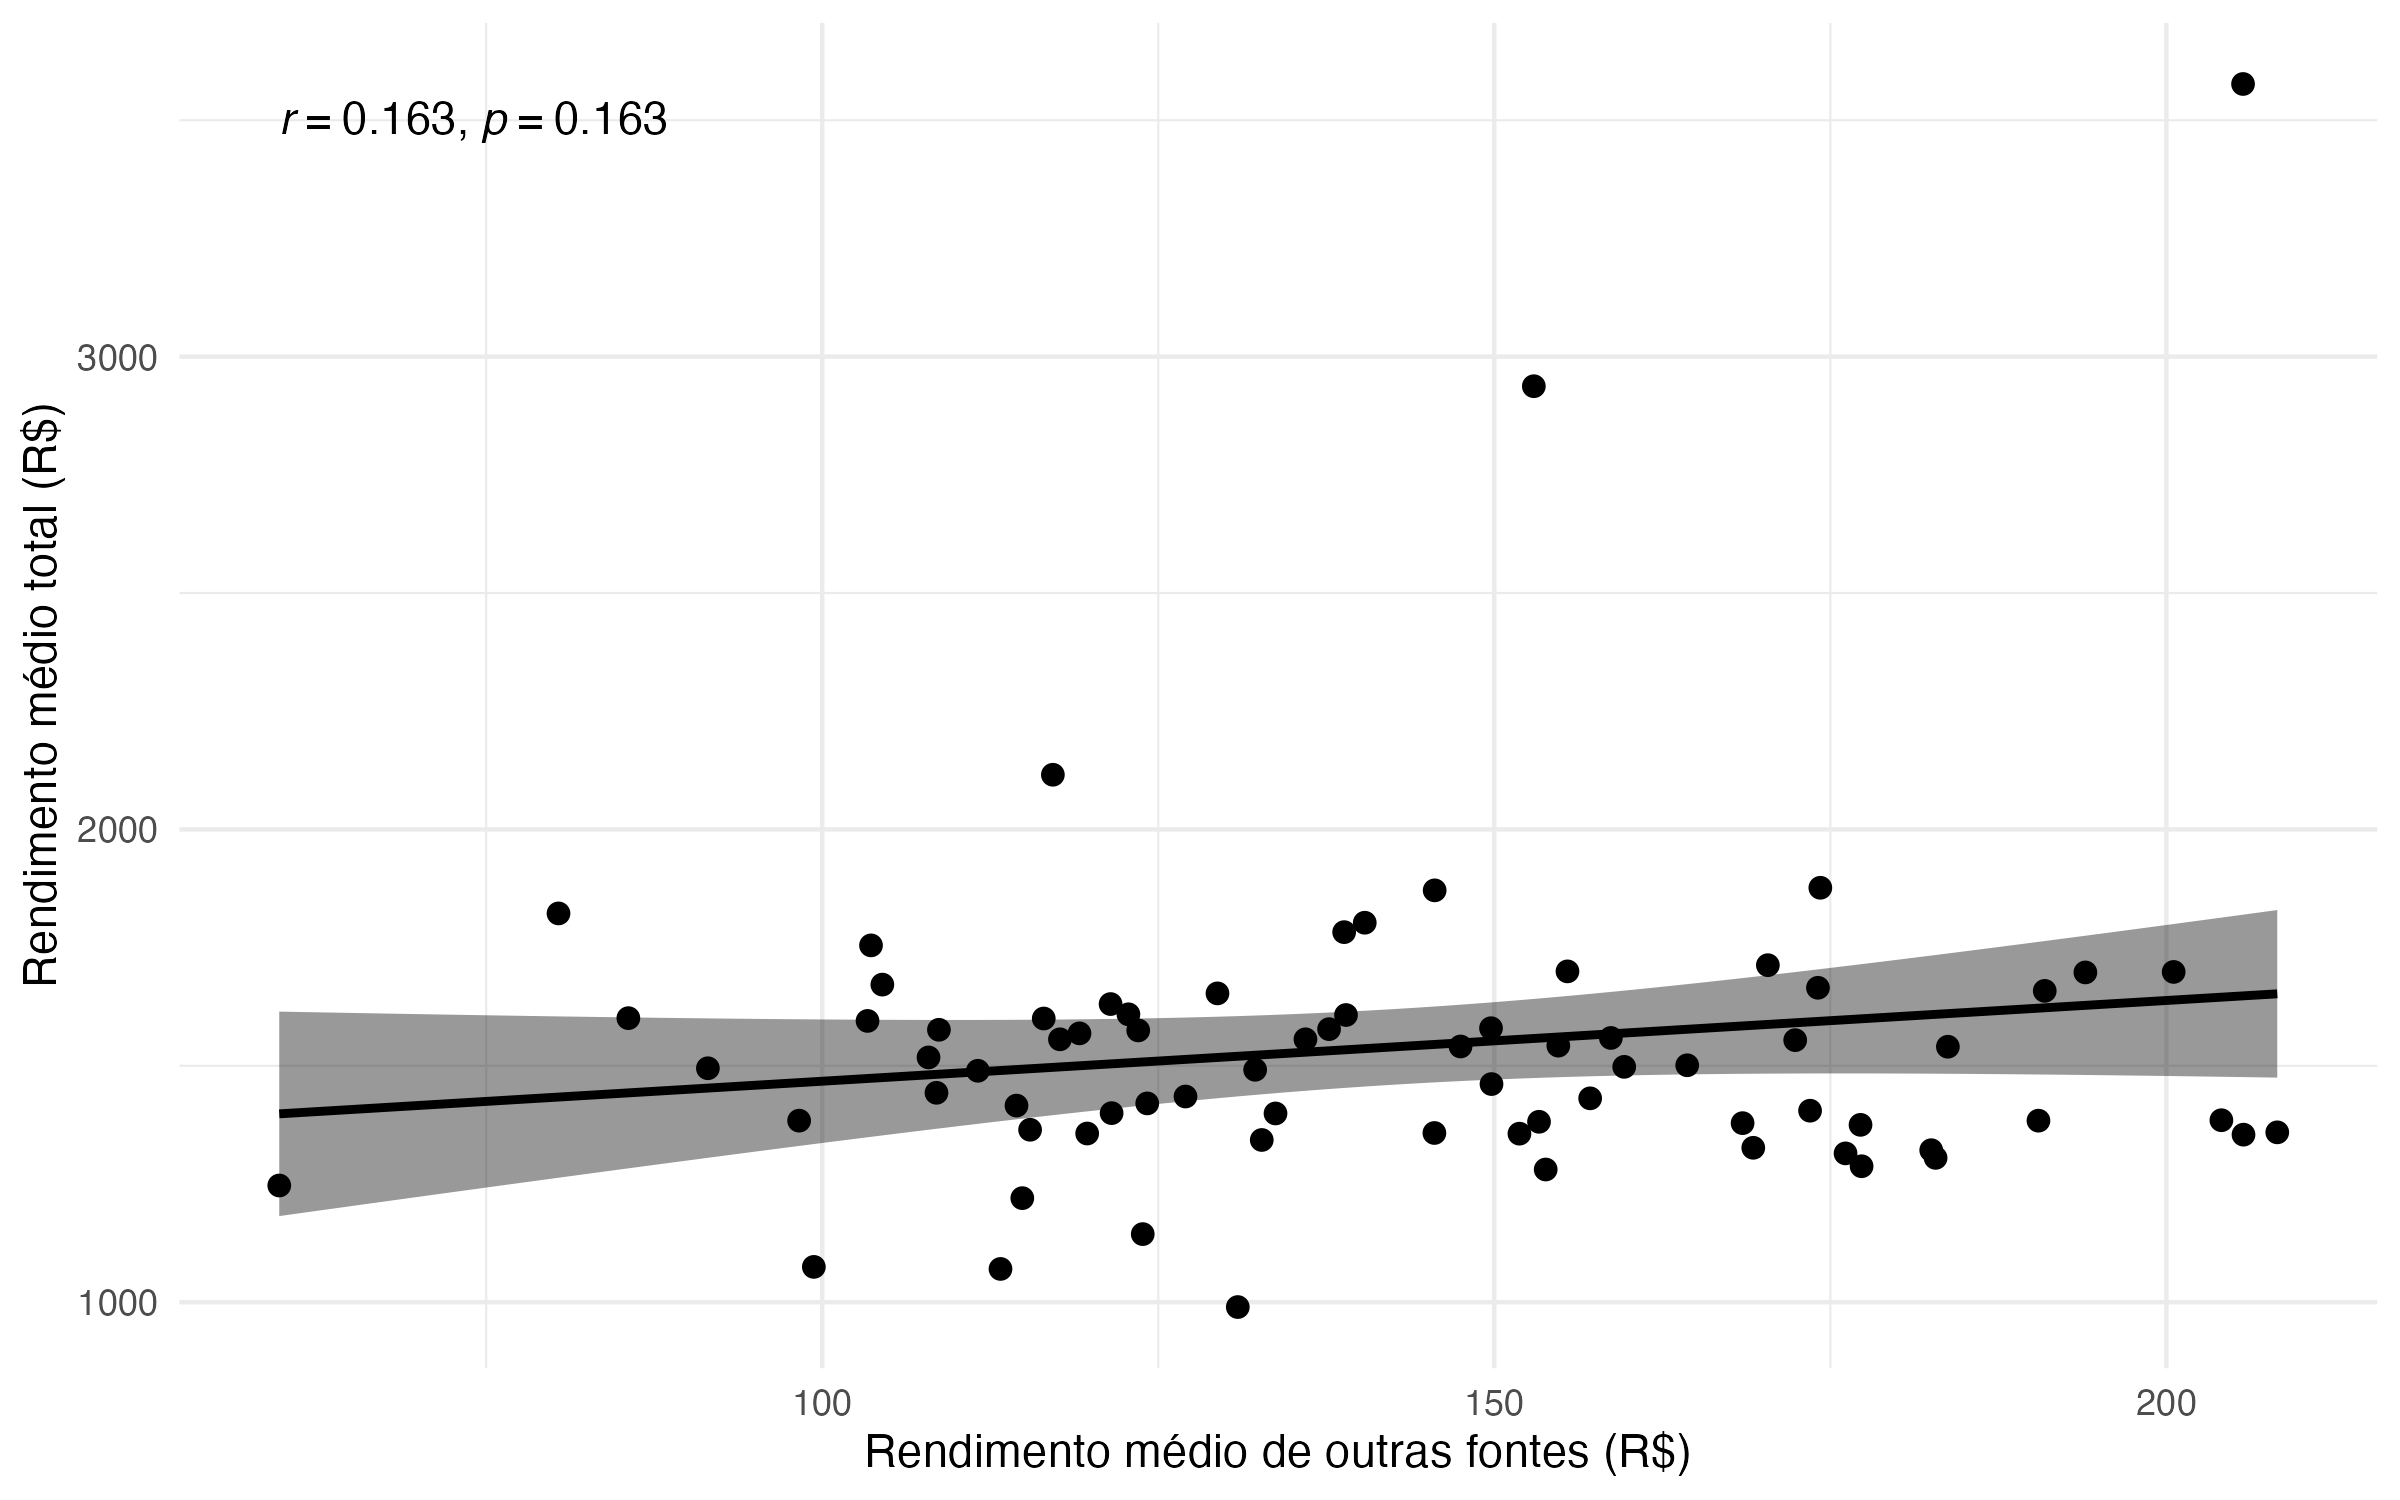
\includegraphics[width=0.85\textwidth]{resultados/item_4b_renda_transferencias_total.png}
    \caption{Rendimento médio total e rendimento médio de transferências e outras fontes por município, Sergipe, 2022}
    \label{fig:item4-renda-transferencias}
    \fonte{Elaboração própria com base nos microdados do Censo Demográfico 2022.}
    \nota{A linha representa o ajuste linear e a faixa sombreada, seu intervalo de confiança de 95\%.}
\end{figure}

\subsection{Participação de outras fontes de renda}

Os maiores percentuais de rendimentos de outras fontes foram observados em Macambira, Pedrinhas, Gararu, conforme a Tabela~\ref{tab:item5-outras-fontes}. A correlação de Pearson entre o rendimento total médio e a participação dessas fontes, apresentada na Figura~\ref{fig:item5-total-participacao}, foi $r = -0{,}468$ ($p < 0{,}001$). A associação negativa indica que municípios com maior rendimento total tendem a apresentar menor participação relativa de outras fontes; portanto, essa participação é relativamente mais elevada em municípios de menor rendimento. Isso não demonstra, por si só, dependência da economia municipal em relação ao governo: P1100 reúne outras fontes de renda sem permitir separar aposentadorias, pensões, PBF ou demais componentes, e a correlação municipal não estabelece causalidade.

\begin{table}[htbp]
\centering
\caption{Municípios com maior participação de rendimentos de outras fontes, Sergipe, 2022}
\label{tab:item5-outras-fontes}
\small
\begin{tabular}{lrrr}
\toprule
Município & Rendimento total médio (R\$) & Outras fontes médias (R\$) & Participação (\%) \\
\midrule
Macambira & 1.359,26 & 208,25 & 15,32 \\
Pedrinhas & 1.354,33 & 205,74 & 15,19 \\
Gararu & 1.384,90 & 204,09 & 14,74 \\
\bottomrule
\end{tabular}
\fonte{Elaboração própria com base nos microdados do Censo Demográfico 2022.}
\nota{Participação calculada como a razão entre P1100 e P1110, conforme o procedimento do item 4.}
\end{table}


\begin{figure}[H]
    \centering
    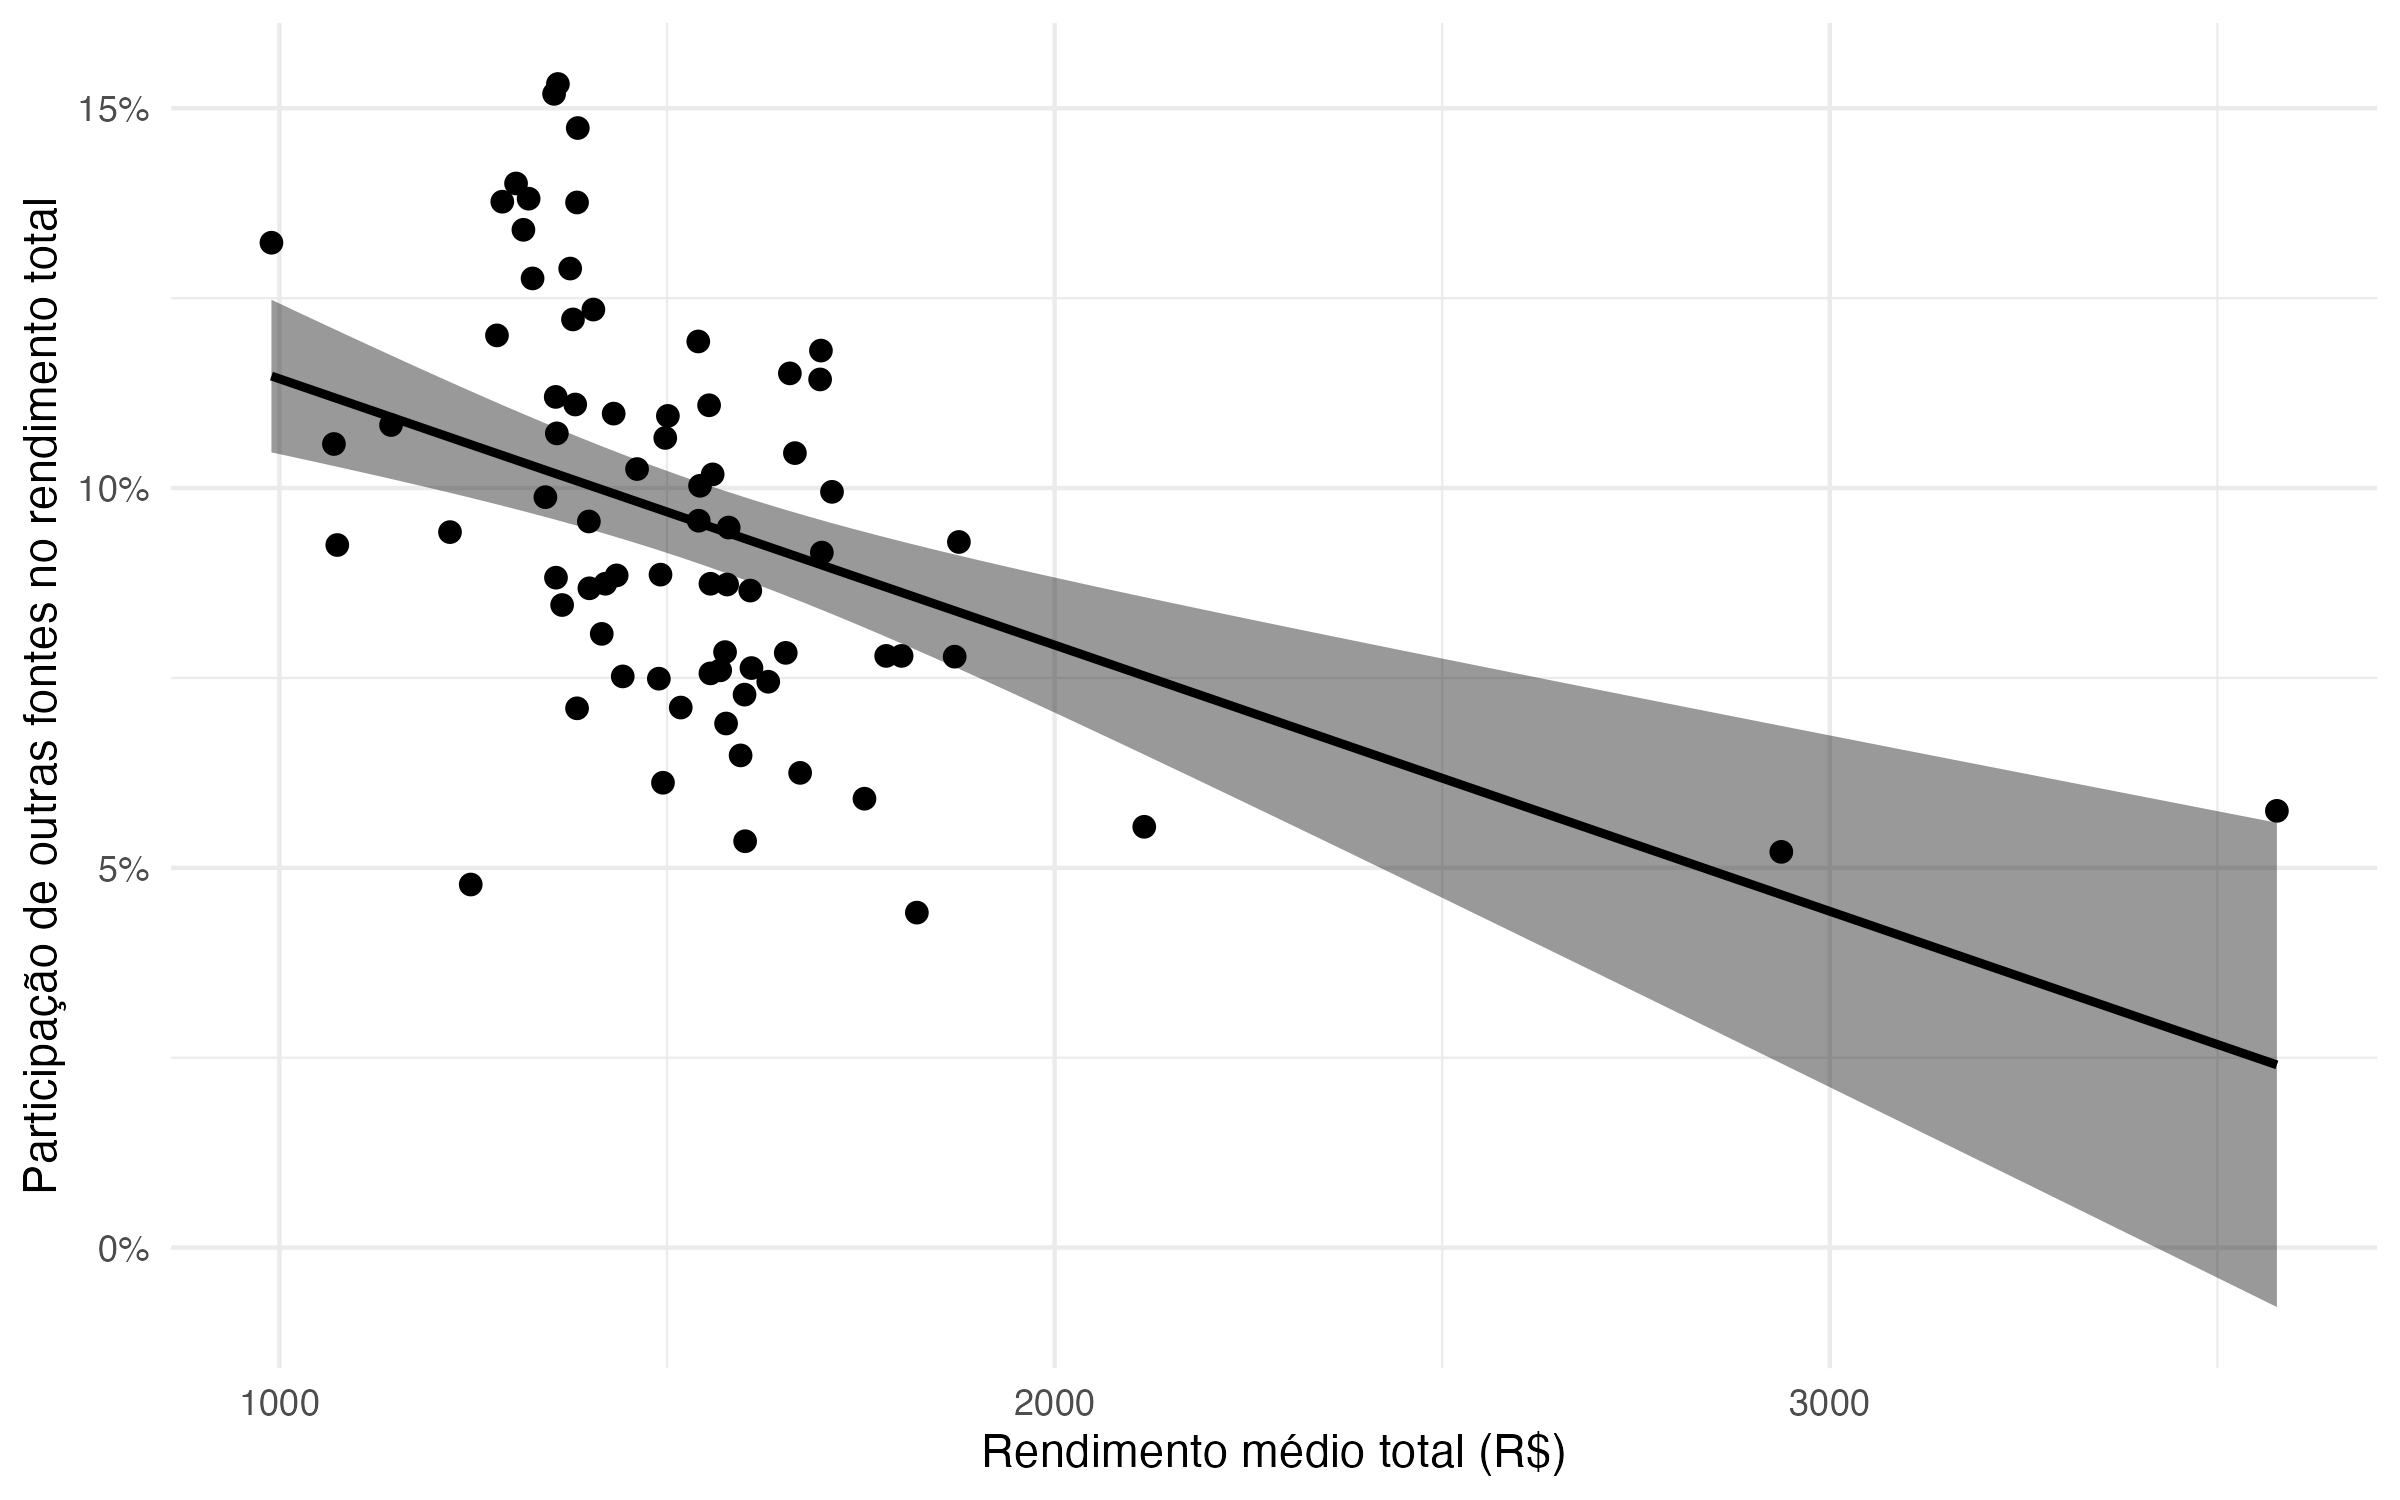
\includegraphics[width=0.85\textwidth]{resultados/item_5_total_participacao_outras_fontes.png}
    \caption{Rendimento médio total e participação de outras fontes por município, Sergipe, 2022}
    \label{fig:item5-total-participacao}
    \fonte{Elaboração própria com base nos microdados do Censo Demográfico 2022.}
    \nota{A linha representa o ajuste linear e a faixa sombreada, seu intervalo de confiança de 95\%.}
\end{figure}

\subsection{Características domiciliares e habitacionais}

\subsubsection{Proporção de domicílios chefiados por mulher}

Em Sergipe, 53,15\% dos domicílios tinham uma mulher como responsável. A Tabela~\ref{tab:item2-1-chefe-mulher} apresenta os três municípios com maiores e menores proporções, ordenados do maior para o menor dentro de cada grupo. A estimativa estadual foi calculada diretamente para o conjunto de domicílios do estado. No nível municipal, a razão de sexo apresentou associação negativa moderada com a proporção de domicílios chefiados por mulheres ($r = -0{,}459; p < 0{,}001$). Assim, municípios com mais homens para cada 100 mulheres tendem a apresentar menor proporção de domicílios com responsável mulher. Essa associação municipal não estabelece causalidade nem descreve necessariamente relações entre indivíduos.

\begin{table}[htbp]
\centering
\caption{Proporção de domicílios chefiados por mulher nos municípios com maiores e menores percentuais, Sergipe, 2022}
\label{tab:item2-1-chefe-mulher}
\small
\begin{tabular}{lr}
\toprule
Município & Domicílios chefiados por mulher (\%) \\
\midrule
\multicolumn{2}{l}{\textbf{Maiores proporções}} \\
Umbaúba & 64,88 \\
Rosário do Catete & 61,60 \\
Santo Amaro das Brotas & 60,24 \\
\midrule
\multicolumn{2}{l}{\textbf{Menores proporções}} \\
Canhoba & 44,43 \\
Telha & 44,23 \\
Gararu & 39,39 \\
\midrule
Sergipe & 53,15 \\
\bottomrule
\end{tabular}
\fonte{Elaboração própria com base nos microdados do Censo Demográfico 2022.}
\nota{Estimativas ponderadas; domicílios identificados pela condição P0170 = 1 e responsáveis mulheres por D0171 = 2.}
\end{table}


\subsubsection{Renda domiciliar per capita por sexo da pessoa responsável}

Em Sergipe, a renda domiciliar per capita média foi de R\$ 1.198,11 nos domicílios com responsável mulher e R\$ 1.559,82 naqueles com responsável homem. A diferença é de R\$ 361,71, e a média dos domicílios com responsável homem é 30,19\% maior. A Tabela~\ref{tab:item2-2-rdpc-sexo} apresenta, para os três municípios com maiores e menores médias de renda no grupo com responsável mulher, as médias dos dois grupos. A Figura~\ref{fig:item2-2-rdpc-seis} compara esses mesmos municípios e marca as médias estaduais. O arquivo CSV em resultados contém as estimativas dos 75 municípios.

\begin{table}[htbp]
\centering
\caption{Renda domiciliar per capita por sexo da pessoa responsável nos municípios com maiores e menores médias femininas, Sergipe, 2022}
\label{tab:item2-2-rdpc-sexo}
\small
\begin{tabular}{lrr}
\toprule
Município & Responsável mulher (R\$) & Responsável homem (R\$) \\
\midrule
\multicolumn{3}{l}{\textbf{Maiores médias entre domicílios com responsável mulher}} \\
Aracaju & 2.019,85 & 2.809,23 \\
Barra dos Coqueiros & 1.486,98 & 2.138,42 \\
São Cristóvão & 1.123,64 & 1.505,71 \\
\midrule
\multicolumn{3}{l}{\textbf{Menores médias entre domicílios com responsável mulher}} \\
Indiaroba & 623,64 & 865,73 \\
Santa Rosa de Lima & 607,04 & 807,75 \\
Brejo Grande & 582,73 & 781,80 \\
\midrule
Sergipe & 1.198,11 & 1.559,82 \\
\bottomrule
\end{tabular}
\fonte{Elaboração própria com base nos microdados do Censo Demográfico 2022.}
\nota{Estimativas ponderadas de renda domiciliar per capita (D0360), segundo o sexo da pessoa responsável (P0160).}
\end{table}


\begin{figure}[H]
    \centering
    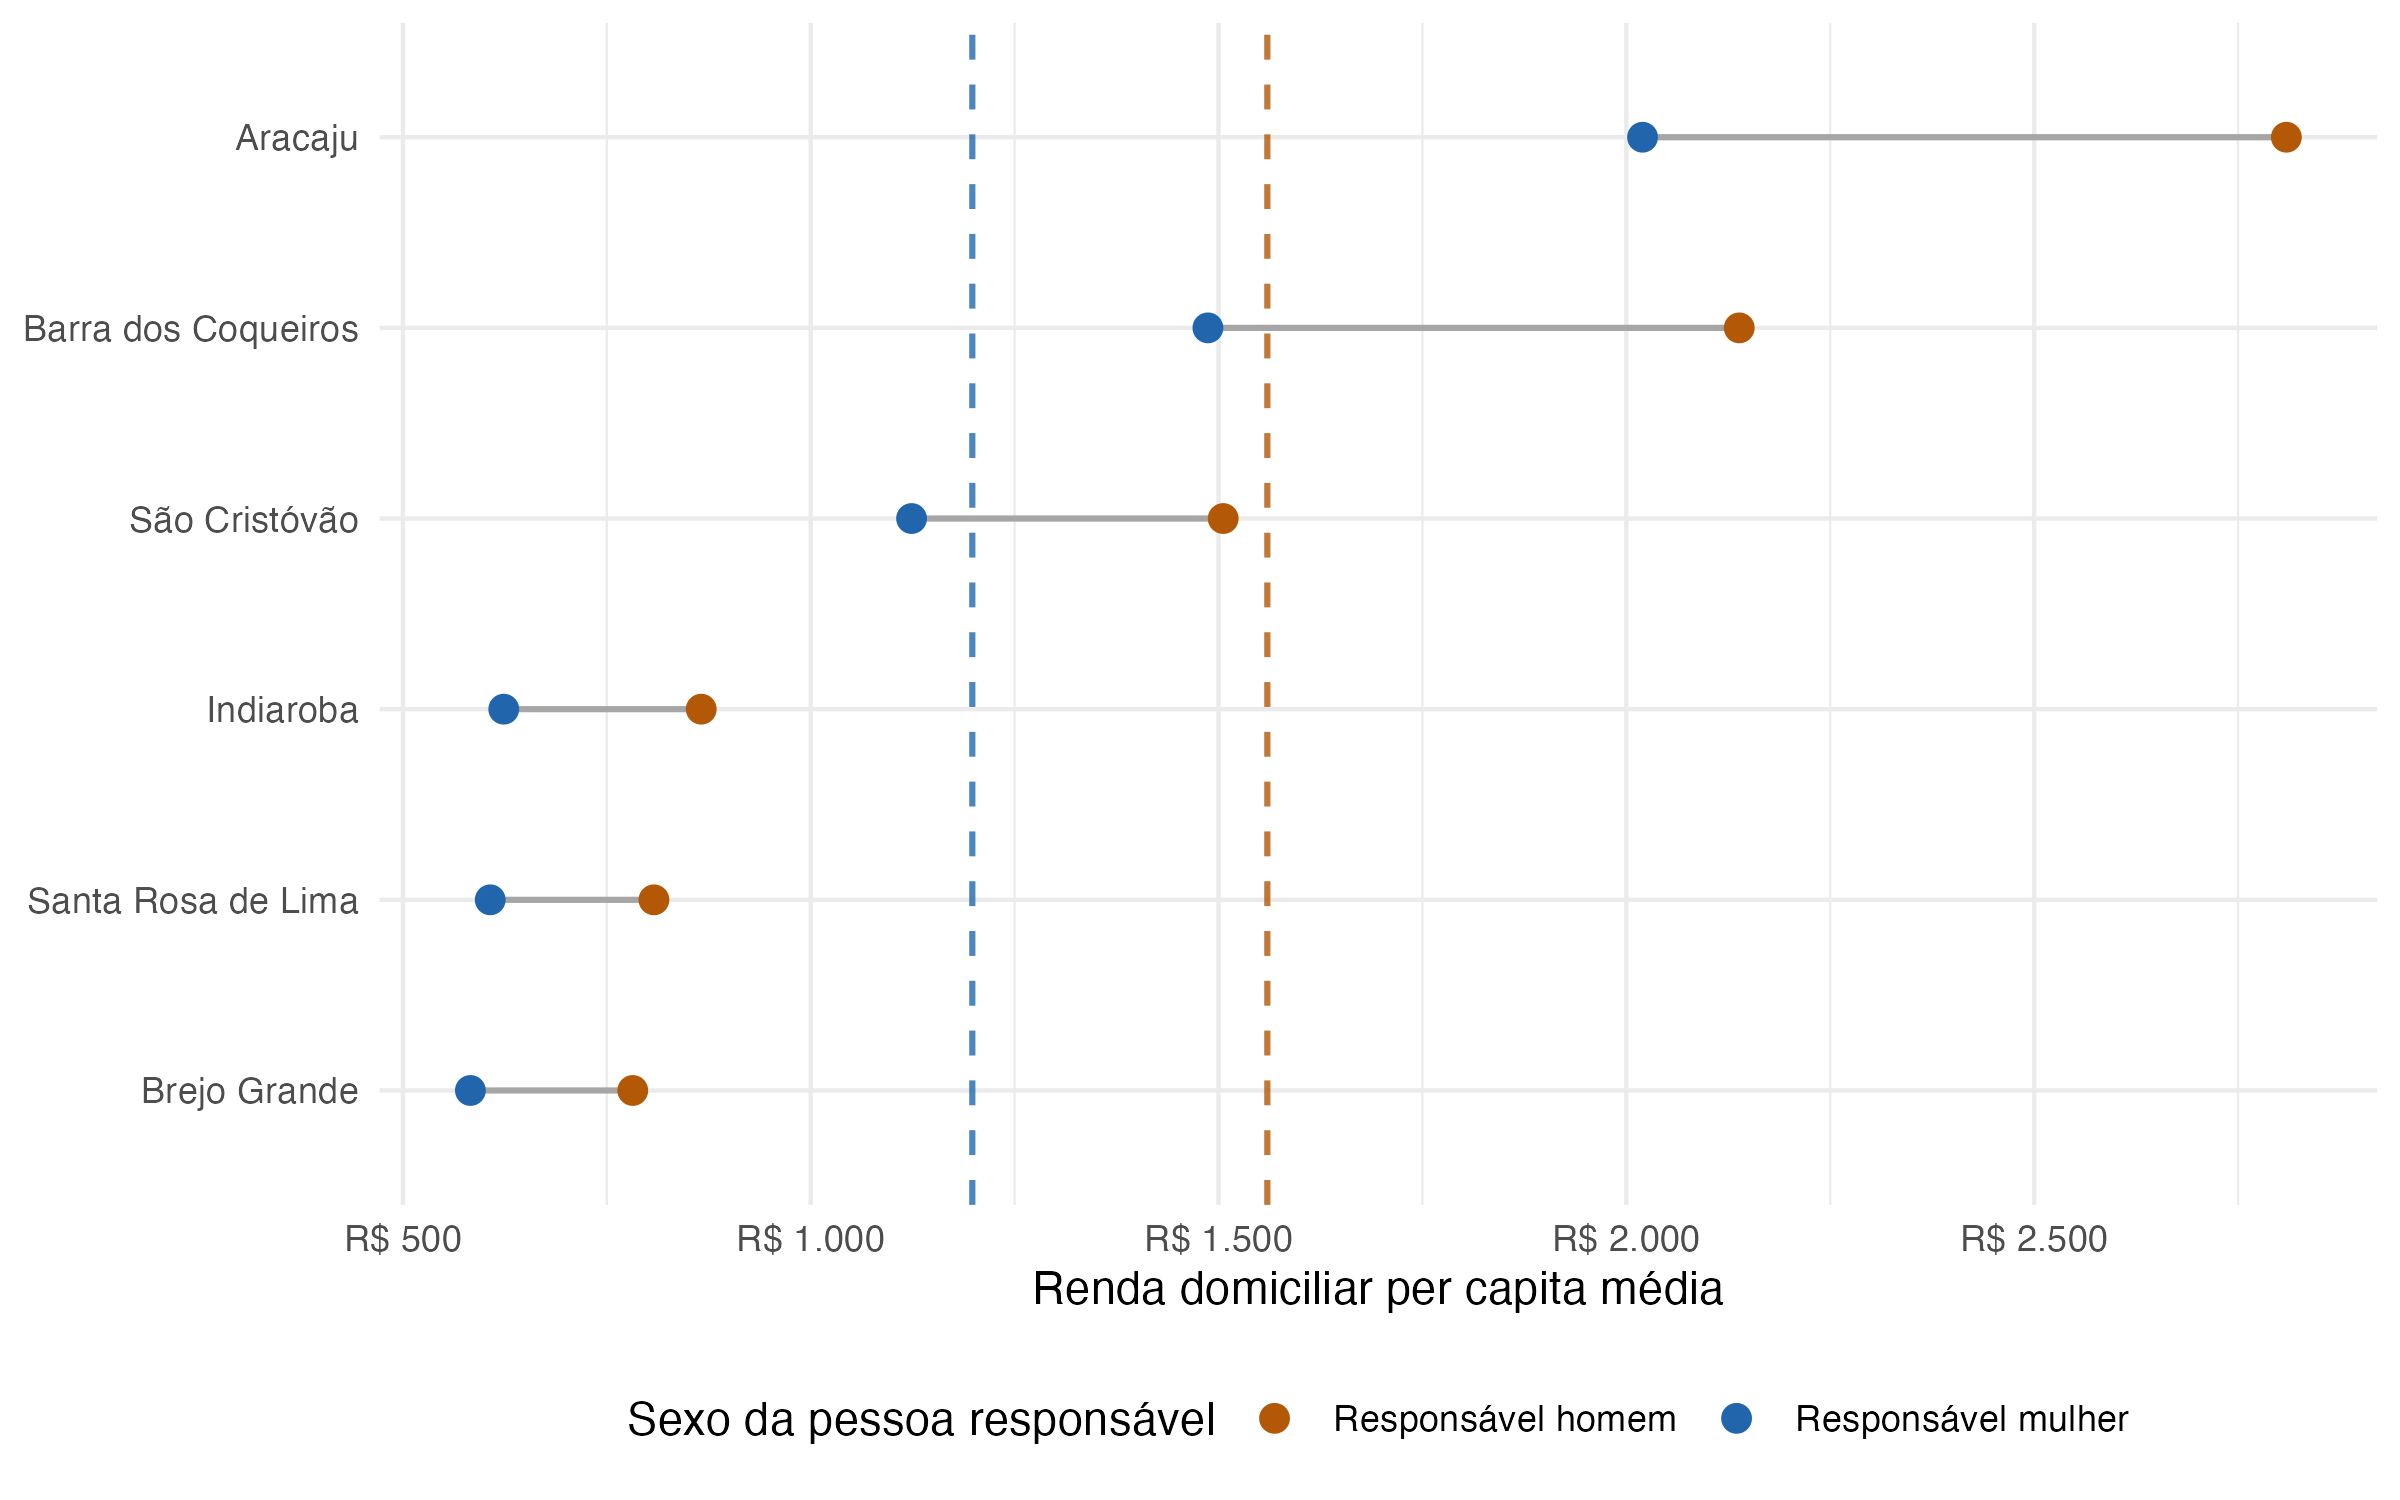
\includegraphics[width=0.9\textwidth]{resultados/item_2_2_rdpc_seis_municipios.png}
    \caption{Renda domiciliar per capita por sexo da pessoa responsável nos seis municípios selecionados, Sergipe, 2022}
    \label{fig:item2-2-rdpc-seis}
    \fonte{Elaboração própria com base nos microdados do Censo Demográfico 2022.}
    \nota{Os pontos estão ligados por município. As linhas tracejadas indicam as médias estaduais de cada grupo.}
\end{figure}

\subsubsection{Municípios com menor renda em domicílios com responsável mulher}

A Tabela~\ref{tab:item2-3-menor-rdpc-mulher} apresenta os dez municípios com menores médias de renda domiciliar per capita nos domicílios com responsável mulher, ordenados do maior para o menor entre os dez selecionados. Os valores variam de R\$ 694,12 em Pedra Mole a R\$ 582,73 em Brejo Grande. Todos os dez municípios ficam abaixo da média estadual de R\$ 1.198,11.

\begin{table}[htbp]
\centering
\caption{Dez municípios com menores rendas domiciliares per capita em domicílios com responsável mulher, Sergipe, 2022}
\label{tab:item2-3-menor-rdpc-mulher}
\small
\begin{tabular}{rlr}
\toprule
Posição & Município & Renda domiciliar per capita (R\$) \\
\midrule
1 & Pedra Mole & 694,12 \\
2 & Porto da Folha & 689,53 \\
3 & Pacatuba & 682,36 \\
4 & Itaporanga d'Ajuda & 663,94 \\
5 & Santa Luzia do Itanhy & 650,39 \\
6 & Poço Redondo & 649,64 \\
7 & Ilha das Flores & 639,48 \\
8 & Indiaroba & 623,64 \\
9 & Santa Rosa de Lima & 607,04 \\
10 & Brejo Grande & 582,73 \\
\bottomrule
\end{tabular}
\fonte{Elaboração própria com base nos microdados do Censo Demográfico 2022.}
\nota{A seleção considera os dez menores valores; a tabela os apresenta em ordem decrescente, conforme a orientação do exercício.}
\end{table}


\subsubsection{Maiores hiatos de renda domiciliar per capita}

O hiato foi calculado subtraindo a renda domiciliar per capita média dos domicílios com responsável mulher da média daqueles com responsável homem. A Tabela~\ref{tab:item2-4-maiores-hiatos-rdpc} apresenta os dez municípios com maiores diferenças absolutas, em ordem decrescente. Entre eles, o maior hiato foi de R\$ 789,37 em Aracaju.

\begin{table}[htbp]
\centering
\caption{Dez maiores hiatos absolutos de renda domiciliar per capita segundo sexo da pessoa responsável, Sergipe, 2022}
\label{tab:item2-4-maiores-hiatos-rdpc}
\small
\begin{tabular}{rlrrr}
\toprule
Posição & Município & Resp. mulher (R\$) & Resp. homem (R\$) & Hiato (R\$) \\
\midrule
1 & Aracaju & 2.019,85 & 2.809,23 & 789,37 \\
2 & Barra dos Coqueiros & 1.486,98 & 2.138,42 & 651,44 \\
3 & São Cristóvão & 1.123,64 & 1.505,71 & 382,07 \\
4 & Rosário do Catete & 719,48 & 1.074,16 & 354,68 \\
5 & Santo Amaro das Brotas & 788,98 & 1.111,90 & 322,92 \\
6 & Carmópolis & 769,38 & 1.075,72 & 306,34 \\
7 & Itabaiana & 1.070,28 & 1.367,85 & 297,57 \\
8 & Nossa Senhora do Socorro & 806,32 & 1.095,68 & 289,36 \\
9 & Carira & 721,61 & 1.002,37 & 280,76 \\
10 & Itaporanga d'Ajuda & 663,94 & 941,88 & 277,93 \\
\bottomrule
\end{tabular}
\fonte{Elaboração própria com base nos microdados do Censo Demográfico 2022.}
\nota{Hiato calculado como renda per capita média de domicílios com responsável homem menos a de domicílios com responsável mulher.}
\end{table}


\subsubsection{Água encanada até dentro da moradia}

Em Sergipe, 93,02\% dos domicílios tinham água encanada até dentro da moradia. A Tabela~\ref{tab:item2-5-agua-encanada} apresenta os dez municípios com menores proporções, do menor para o maior. O menor percentual foi de 69,64\% em Pinhão.

\begin{table}[H]
\centering
\caption{Dez municípios com menores proporções de domicílios com água encanada até dentro da moradia, Sergipe, 2022}
\label{tab:item2-5-agua-encanada}
\small
\begin{tabular}{rlr}
\toprule
Posição & Município & Água encanada dentro da moradia (\%) \\
\midrule
1 & Pinhão & 69,64 \\
2 & Tomar do Geru & 73,34 \\
3 & Simão Dias & 74,19 \\
4 & Riachão do Dantas & 74,49 \\
5 & Macambira & 74,81 \\
6 & Gararu & 74,93 \\
7 & Poço Redondo & 75,69 \\
8 & Monte Alegre de Sergipe & 75,73 \\
9 & Carira & 75,79 \\
10 & Siriri & 77,16 \\
\midrule
\multicolumn{2}{l}{Sergipe} & 93,02\% \\
\bottomrule
\end{tabular}
\fonte{Elaboração própria com base nos microdados do Censo Demográfico 2022.}
\nota{Domicílio contado como atendido quando D0300 = 1, isto é, a água chega encanada até dentro da moradia.}
\end{table}


\subsubsection{Esgotamento sanitário inadequado}

Em Sergipe, 32,96\% dos domicílios foram classificados com esgotamento sanitário inadequado. A variável D0250 registra o destino do esgoto do banheiro; o valor 3 corresponde a fossa séptica ou fossa-filtro não ligada à rede. Neste laboratório, foram considerados inadequados os domicílios cujo valor de D0250 é superior a 3 \cite{ibgedicmicrodados2022}. A Tabela~\ref{tab:item2-6-esgoto-inadequado} apresenta os três municípios com maiores e menores proporções; em cada grupo, os valores estão ordenados do maior para o menor. A maior proporção foi de 98,19\% em Areia Branca.

\begin{table}[H]
\centering
\caption{Proporção de domicílios com esgotamento sanitário inadequado nos municípios com maiores e menores percentuais, Sergipe, 2022}
\label{tab:item2-6-esgoto-inadequado}
\small
\begin{tabular}{lr}
\toprule
Município & Esgotamento inadequado (\%) \\
\midrule
\multicolumn{2}{l}{\textbf{Maiores proporções}} \\
Areia Branca & 98,19 \\
Arauá & 96,87 \\
Cristinápolis & 96,59 \\
\midrule
\multicolumn{2}{l}{\textbf{Menores proporções}} \\
Pacatuba & 10,61 \\
Santa Rosa de Lima & 6,98 \\
Aracaju & 5,42 \\
\midrule
Sergipe & 32,96 \\
\bottomrule
\end{tabular}
\fonte{Elaboração própria com base nos microdados do Censo Demográfico 2022.}
\end{table}


\subsubsection{Internet e esgotamento sanitário}

Sim. Em 64 dos 75 municípios, a proporção de domicílios com acesso à internet (D0330 igual a 1) supera a proporção com esgotamento considerado adequado pelo critério do exercício, que classifica como adequados os valores da variável D0250 até 3. Em Sergipe, as proporções são de 81,34\% para internet e 67,04\% para esgotamento adequado, diferença de 14,30 pontos percentuais. A Tabela~\ref{tab:item2-7-internet-esgoto} mostra os municípios com as maiores diferenças positivas e aqueles em que as proporções são mais próximas, mas ainda há mais cobertura de internet. Há também diferenças no modo de provisão: a família pode contratar internet de um provedor quando existe cobertura; já ampliar a rede coletora de esgoto até as residências exige infraestrutura coletiva e decisões de planejamento e investimento público. Além disso, o critério adotado considera adequada a fossa séptica ou fossa-filtro não ligada à rede (valor 3 de D0250), de modo que a medida não representa apenas o alcance da rede coletora. O contraste evidencia desigualdade territorial entre serviços essenciais, mas os dados agregados por município não permitem concluir que as famílias tenham escolhido internet em vez de saneamento.

\begin{table}[H]
\centering
\caption{Diferença entre a proporção de domicílios com internet e com esgotamento adequado, Sergipe, 2022}
\label{tab:item2-7-internet-esgoto}
\small
\begin{tabular}{lrrr}
\toprule
Município & Internet (\%) & Esgotamento adequado (\%) & Diferença (p.p.) \\
\midrule
\multicolumn{4}{l}{\textbf{Maiores diferenças positivas}} \\
Santana do São Francisco & 81,72 & 3,53 & 78,19 \\
Areia Branca & 78,88 & 1,81 & 77,07 \\
Muribeca & 75,72 & 6,13 & 69,59 \\
\midrule
\multicolumn{4}{l}{\textbf{Menores diferenças positivas}} \\
São Miguel do Aleixo & 64,45 & 61,80 & 2,65 \\
Rosário do Catete & 83,64 & 83,03 & 0,61 \\
Carmópolis & 84,52 & 84,30 & 0,22 \\
\midrule
Sergipe & 81,34 & 67,04 & 14,30 \\
\bottomrule
\end{tabular}
\fonte{Elaboração própria com base nos microdados do Censo Demográfico 2022.}
\nota{Esgotamento considerado adequado para valores da variável D0250 até 3, seguindo o critério do exercício, incluindo fossa séptica ou fossa-filtro não ligada à rede (valor 3); diferença em pontos percentuais.}
\end{table}



\section{Considerações finais}

Os resultados mostram desigualdades municipais nas dimensões demográfica, econômica e domiciliar. A taxa de desocupação variou de 2,38\% a 19,59\%, e a taxa de analfabetismo das pessoas de 15 a 64 anos foi de 9,01\% no estado. As correlações entre razão de sexo, participação do setor primário e ocupação descrevem padrões territoriais, mas não estabelecem causalidade.

Quanto à renda, observa-se desigualdade de gênero: a renda domiciliar per capita média nos domicílios com responsável homem foi 30,19\% maior que nos domicílios com responsável mulher. A participação de outras fontes foi relativamente maior nos municípios com menor rendimento total; porém, P1100 reúne aposentadorias, pensões, benefícios sociais e outras rendas, sem permitir atribuir esse padrão a um componente específico.

Nas condições domiciliares, 93,02\% dos domicílios tinham água encanada dentro da moradia e 32,96\% foram classificados com esgotamento inadequado. Em 64 dos 75 municípios, a cobertura de internet superou a de esgotamento adequado. Os serviços têm modos distintos de provisão: a família pode contratar internet onde há cobertura, enquanto expandir a rede coletora exige infraestrutura coletiva e investimento público. Além disso, o critério de esgotamento adequado inclui fossa séptica ou fossa-filtro não ligada à rede, portanto não mede apenas o alcance da rede coletora.

Em conjunto, a análise oferece um retrato comparativo das condições de vida nos municípios sergipanos. As estimativas descrevem o contexto de 2022: correlações municipais não demonstram causalidade, e diferenças agregadas não revelam escolhas individuais das famílias.


\renewcommand{\refname}{\centering REFERÊNCIAS}

{\singlespacing
\clearpage
\bibliography{references}
\addcontentsline{toc}{section}{REFERÊNCIAS}
}
\end{document}
